% Chapter X

\chapter{Données clinique}

\label{ch:02-02} % For referencing the chapter elsewhere, use \autoref{ch:name} 
%----------------------------------------------------------------------------------------

% \section{}

La fonction de CFTR est de réguler le transport des ions et les mouvements d’eau au travers de la barrière épithéliale des cellules qui produisent du mucus, de la sueur ou de la salive. Sans altération CFTR fonctionne comme un canal à travers la membrane et transporte les ions chlorure négativement chargé en dehors de la cellule afin d’aider au contrôle des mouvements d’eau dans les tissus, élément nécessaire pour la production d’un fin mucus qui va protéger les voies aériennes, le système digestif et reproducteur, ainsi que d’autre organes et tissues.

Parmi les organes atteints par la mucoviscidose, les atteintes pulmonaires sont les plus graves car elles se révèlent fatal dans la plupart des cas. Succinctement, le gène CFTR défectueux est à l’origine d’une absorption de l’eau contenue dans le mucus qui protège les voies respiratoires. Cette couche fine devenue visqueuse empêche les cellules ciliaires de battre et donc les mécanismes d’évacuation du mucus de fonctionner correctement. Ainsi, l’ensemble des particules inhalées reste retenues à la surface des voies aériennes et des bactéries trouvent ainsi un environnement favorable à leurs proliférations.

Les atteintes pancréatiques, elles, vont avoir pour conséquence une difficulté d’assimilation des nutriments, le pancréas très abîmé de naissance et encombré par un épaississement du mucus empêche la bonne libération des enzymes essentielles à une bonne digestion. Le foie et le système digestif atteint aussi, peuvent présenter une cirrhose biliaire pour le premier et une constipation et obstruction intestinale pour le second. Un retard de la puberté et une infertilité peut aussi toucher certains patients (Figure \ref{organe}).

On peut observer une large diversité d’expression clinique d’un patient à l’autre, que ce soit pour l’âge d’apparition des premiers symptômes ou la sévérité de l’évolution de la maladie mais un déclin des fonctions pulmonaire caractérisé par une infection progressive des voies respiratoires ainsi qu’une inflammation reste la cause principale de mortalité et morbidité.

\begin{center}
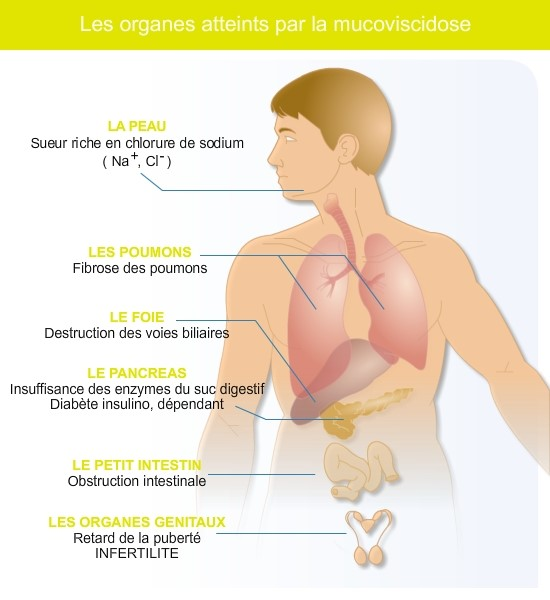
\includegraphics[scale=0.5]{gfx/organes.jpg} 
\captionsetup{type=figure}
\captionof{figure}{organes atteints par la Mucoviscidose}
       \label{organe}
\end{center}
